\documentclass[12pt]{article}
\usepackage{amsmath,amsfonts,amssymb}
\usepackage{ctex}
\usepackage{graphicx}
\usepackage{geometry}
\geometry{margin=1in}
\usepackage{float}
\usepackage{listings}
\usepackage{xcolor}
\definecolor{codegray}{gray}{0.9}
\lstset{
  backgroundcolor=\color{codegray},
  basicstyle=\ttfamily\small,
  breaklines=true
}

\title{数值分析 HW06 (week07) 实验报告}
\author{学号: PB22000150\quad 姓名: 刘行}
\date{\today}

\begin{document}

\maketitle

	\section{实验一: Richardson 外推法求导数}
		\subsection{实验原理}
			Richardson 外推法通过对差分公式中的步长 $h$ 进行多次减半, 构造出逼近导数的三角阵列, 通过消除主误差项, 从而提高导数逼近的精度. 基本思想是:
			\[ D(h) = D + C_1 h^p + C_2 h^{p+1} + \cdots \]
			通过多次计算 $D(h), D(h/2), \dots$ 并进行外推, 最终获得高精度导数近似.

		\subsection{代码分析}
			程序算法部分分为三个函数模块: 基本差商函数, 外推公式, 三角阵生成函数. 算法函数最终在 \texttt{main\_code4.m} 脚本文件中调用.

		\subsection{实验结果}
			对三个函数分别计算导数, 输出三角阵结果如下:

\begin{lstlisting}
For f(x) = @(x)log(x), x = 3.00, M = 3:
	0.2877         0         0         0
	0.3083    0.3152         0         0
	0.3202    0.3241    0.3247         0
	0.3266    0.3287    0.3290    0.3291
			
For f(x) = @(x)tan(x), x = 0.931, M = 4:
   -4.0185         0         0         0         0
   11.1747   16.2391         0         0         0
	4.3017    2.0106    1.0621         0         0
	3.3543    3.0385    3.1071    3.1395         0
	3.0346    2.9280    2.9207    2.9177    2.9169
			
For f(x) = @(x)sin(x^2+(1/3)*x), x = 0.00, M = 5:
	0.9719         0         0         0         0         0
	0.8094    0.7553         0         0         0         0
	0.5813    0.5052    0.4885         0         0         0
	0.4581    0.4170    0.4111    0.4099         0         0
	0.3958    0.3750    0.3722    0.3716    0.3715         0
	0.3646    0.3542    0.3528    0.3525    0.3524    0.3524
\end{lstlisting}

			其中真实导数值分别是 $0.3333$, $2.7778$, $0.3333$. 可以看到在此 M 值下, 外推法的结果与真实值还有一定差距.

		\subsection{结果分析}
			结果显示, 随着 $M$ 增大, 外推结果趋于稳定, 误差大幅减少, 验证了外推法通过误差抵消提升精度的理论基础.

	\section{实验二: 复化梯形与Simpson积分法}
		\subsection{实验原理}
			将积分区间划分为 $N$ 等小区间, 对每个小区间分别应用梯形或Simpson积分规则, 得到整体积分近似. 误差满足:
			\[ E_T \sim O\left(\frac{1}{N^2}\right), \quad E_S \sim O\left(\frac{1}{N^4}\right) \]

		\subsection{代码分析}
			分别实现两个复化积分函数, 并对误差进行计算. 之后对比误差结果.

		\subsection{实验结果}
			对 $\int_0^4 \sin x\,dx$ 和 $\int_0^{2\pi} \sin x\,dx$, 用 $N = 2^k, k=1,\dots,12$ 进行积分和误差分析. 结果输出较长, 这里仅展示 $k = 12$ 时的误差表格以及收敛阶表格:
\begin{lstlisting}
a = 0.0000, b = 4.0000
	k = 12, N = 4096
	Trapezoidal: I = 1.6536  Error = 1.3142e-07
	Simpson:     I = 1.6536  Error = 8.2157e-15

Order (Trapezoidal):
    2.0782    2.0184    2.0045    2.0011    2.0003    2.0001    2.0000    2.0000    2.0000    2.0000    2.0000

Order (Simpson):
    4.6789    4.1367    4.0327    4.0081    4.0020    4.0005    4.0001    4.0000    4.0000    3.9954    4.0290

a = 0.0000, b = 6.2832
	k = 12, N = 4096
	Trapezoidal: I = 0.0000  Error = 1.8048e-16
	Simpson:     I = 0.0000  Error = 3.8515e-17

Order (Trapezoidal):
  -Inf   -0.7906    1.5612   -2.1865    2.3564    2.9649   -4.2685    3.0560   -1.4457   -1.1969   -0.2566

Order (Simpson):
   Inf      -Inf    0.3418    2.6110   -0.8791   -1.2655   -0.2918    0.1362    2.2536   -2.2491    1.5703
\end{lstlisting}

		\subsection{结果分析}
			从结果可以看出, 复化Simpson法的收敛阶比复化梯形法高, 误差更小. 但在某些情况下, 如 $\int_0^{2\pi} \sin x\,dx$, 两者的收敛阶都比较混乱, 可能是函数的周期性导致的.

	\section{实验三: Lagrange 插值积分逼近}
		\subsection{实验原理}
			利用 Lagrange 插值多项式 $p_L(x)$ 对函数 $f(x)$ 进行插值, 再对插值多项式积分, 得到对原函数积分的逼近. 节点选取两种方式:
			\begin{enumerate}
				\item 等距节点: $x_{i} = 1 - \frac{2i}{N}$
				\item Chebyshev 节点: $x_{i} = -\cos\left(\frac{i + 1}{N + 2}\pi\right)$
			\end{enumerate}

		\subsection{代码分析}
			核心是构造 Lagrange 基函数并积分. 插值使用逐项构造, 积分使用 \texttt{poly()} 函数通过零点求出多项式系数, 最终直接使用 Newton-Leibniz 公式求出多项式的积分.

		\subsection{实验结果}
			对 $f(x) = \frac{1}{1 + 25x^2}$, 计算

			\begin{equation*}
				\int_{-1}^{1} f(x) dx \approx \int_{-1}^{1} p_L(x) dx
			\end{equation*}

			比较不同节点方式, 不同 $N=5,10,\dots,40$ 下的误差. 结果如下:
\begin{lstlisting}
等距节点结果:
N	PolyIntegral	FuncIntegral	Error
5	0.46153846		0.54936031		8.78e-02
10	0.93466011		0.54936031		3.85e-01
15	0.83111180		0.54936031		2.82e-01
20	-5.36991053		0.54936031		5.92e+00
25	-5.39964172		0.54936031		5.95e+00
30	153.79560807	0.54936031		1.53e+02
35	176.15316097	0.54936031		1.76e+02
40	13309.89202652	0.54936031		1.33e+04
	
Chebyshev 节点结果:
N	PolyIntegral	FuncIntegral	Error
5	0.48114044		0.54936031		6.82e-02
10	0.55408569		0.54936031		4.73e-03
15	0.54758613		0.54936031		1.77e-03
20	0.55001079		0.54936031		6.50e-04
25	0.54935859		0.54936031		1.72e-06
30	0.54907809		0.54936031		2.82e-04
35	0.51280829		0.54936031		3.66e-02
40	-0.54029973		0.54936031		1.09e+00
\end{lstlisting}


		\subsection{结果分析}
			等距节点误差随 $N$ 增大反而变大 (Runge现象), 而Chebyshev 节点误差迅速减小, 验证了节点选择对插值和积分精度的重要影响.

			对于 Chebyshev 节点, 误差在 $N=25$ 时已经非常小, 之后反而增大, 可能是由于数值计算精度限制. 逐步计算发现, 问题可能出现在多项式系数计算上, 由于 Chebyshev 节点的分布, 当 $N$ 较大时, 多项式的低次项系数会非常小, 导致计算精度下降. 如图所示, 在 $N=40$ 时, 低次项系数已经变为 0, 导致计算误差增大.

			\begin{figure}[htbp]
				\centering
				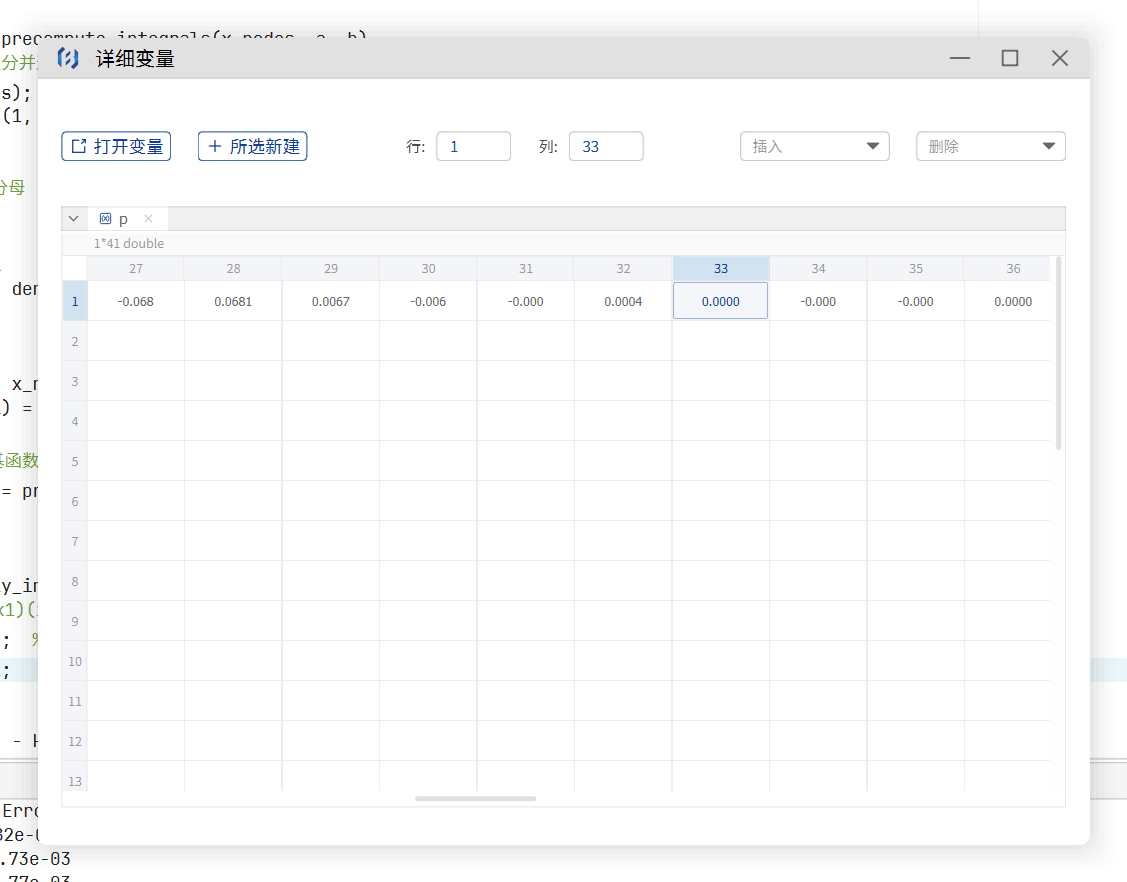
\includegraphics[width=0.8\textwidth]{figure/poly_coeffs.png}
				\caption{Chebyshev 节点 $N=40$ 时 $l_{1}$ 分子部分的多项式系数}
				\label{fig:poly_coeffs}
			\end{figure}

\end{document}
